% INNAN DU COMMITAR!
% Uppdatera datum
% Uppdatera version
%-----
% Document name



\documentclass[10pt,a4paper]{article}
\usepackage[utf8]{inputenc}
\usepackage[english]{babel}
\usepackage{amsmath}
\usepackage{amsfonts}
\usepackage{amssymb}
\usepackage{graphicx}
\usepackage{geometry}

\title{PostCardBuddy}
\author{Team C}

\begin{document}
\begin{titlepage}
\newgeometry{left=2cm,top=1cm,right=2cm}
\newcommand{\HRule}{\rule{\linewidth}{0.5mm}}


\begin{flushright}
November 22, 2015 v1.00\\[3cm]
\end{flushright}


\centering
\textsc{\LARGE Team C}\\[0.5cm]

\HRule \\[0.4cm]
{ \huge \bfseries PostCardBuddy}\\[0.3cm]
{\Large \bfseries Project Experiences}\\[0.4cm] % Title of your document
\HRule \\[1.5cm]

\vfill
\begin{flushleft}
%Authors, write on separate lines
\textit{Authors of this document:}\\
Emma Albertz\\
Caroline Brandberg\\
Linnéa Claesson\\
Billy Johansson\\
Johan Ju\\
Jacob Mejvik\\
Carl Rynegardh
\end{flushleft}

\end{titlepage}
\pagenumbering{gobble}



%\begin{center}
%\textit{\large Version History}
%
%    \begin{tabular}{ | l | l | l | p{5cm} |}
%    \hline
%    \textbf{Version} & \textbf{Date} & \textbf{Responsible} & \textbf{Description} \\ \hline
%    1.0 & 2015-10-14 & EA, LC & Baseline\\ \hline
%    \end{tabular}
%\end{center}



\setcounter{tocdepth}{2}
\tableofcontents
\newpage
\pagenumbering{arabic}

%---------------------------------------------------------------%
% A description of our requirements engineering work, including experiences and reflections in relation to learning objectives.
% The Project Experiences should not include course evaluation issues, but focus on your own work and learning outcome.
%---------------------------------------------------------------%

%-------------------------------------------------------------------%
%-------------- Background -----------------------------------------%
%-------------------------------------------------------------------%
\section{Introduction}
This document aims to describe how the work has been conducted during the project. It also contains the groups reflections on the work process and the difficulties with different parts of the project. 


%-------------------------------------------------------------------%
%--------------- Methods and Techniques ----------------------------%
%-------------------------------------------------------------------%
% Description of the chosen methods/techniques for elicitation, specification, validation, and prioritization.
% Motivation for why you chose the used methods/techniques.
\section{Methods and Techniques}




% 3D) apply more than one elicitation technique in a relevant way.
\subsection{Elicitation}
To find relevant elicitation techniques, \textit{Software Requirements - Styles and Techniques} by Soren Lauesen have been used as a guidance\cite{soren}. A first stakeholder analysis was conducted and the different stakeholders were then approached using different elicitation techniques. 

The following elicitation techniques were used prior to release 1:
\begin{description}
\item[Brainstorming] Used as a first step within the team to come up with basic ideas and functions. During the brainstorming session the functions specified by the key customer were also considered.

\item[Questionnaire] The questionnaire was sent out to people within the end user group. Questions from the brainstorming session were used. People answering where asked to grade functions with grade 0-5, where zero stood for not interesting and five for very interesting. An age field was added to see if there was a difference in interest of various functions between ages. 

\item[Interviews] The key customer was interviewed.

\item[Prototypes] Three team members created one prototype each, independently of each other so as not to affect each other's ideas. It was decided to do this right away due to the time constraint upon this project. The prototypes are meant to be used for ideas to the graphical interface of the application. The use of prototypes is considered a suitable technique for this project since there are many easy to use and free programs available to make them and it gives not only the stakeholders but also the authors of the requirements a good idea of what it should look like and be able to do. It will be specifically be used when eliciting requirements from prospective end users.

\item[Document study] There is already a similar existing application on the market and it was used to further elicit functionality not already thought of and also to perhaps eliminate functionality that intervenes with the user experience. This was done after the initial brainstorming, to avoid making an identical application and not interfere with the team's creativity. This will be done more thoroughly for release 2.

\item[Focus group]

\end{description}


% 4B) use at least four different specification techniques adequately tailored to the context.
\subsection{Specification}

\begin{description}
\item[Context diagram] A context diagram will be used since it is easy to use at the time for validation and verification. The diagram gives a good over-view of the system, both for the use of the client but also for the developers. 
\end{description}

% 3F) to assess the quality of requirements and find relevant problems of several different types.
% 3G) apply more than one validation technique.
% 4G) adapt the validation to the context and provide rationale for the chosen validation techniques.
\subsection{Validation}
\begin{description}
\item[Prototypes] The prototype gives the customer a unique opportunity to validate how the product matches their expectations. The prototypes will be contentiously adapted to the customers' needs and wants and new features will be added (or others removed) so that it becomes a good reflection on where the project is going. % Ta bort kanske?
\end{description}


% 3I) use more than one prioritization technique in a relevant way.
\subsection{Prioritization}

%--------------------------------------------------------------------%
%--------------- Reflections ----------------------------------------%
%--------------------------------------------------------------------%
% Reflection on the usage of these methods/techniques in terms of what was successful and what was challenging. Example questions for reflection: What have you learned in relation to the learning objectives in this course program? What would you have done differently if you would do this project again as a "real" project, based on what you know now? What have you learned in relation to the learning objectives?


% Osäker om detta är rätt placering: 5B) provide motivated estimations of target quality levels using well-defined scales.
% 4F) to find, prioritize and discuss requirements quality problems of different types, while reaching 	beyond form issues.
% 5D) reason about the relation between requirements quality problems and risks, both from a customer and developer viewpoint.
\section{Reflections}

% 3E) reflect on elicitation experiences.
% 4E) reason about the need for further elicitation in relation to specification quality.
% 5C) go beyond initial stakeholders and given frames, while challenging the domain boundaries and eliciting creative ideas and deep domain knowledge in real-world contexts.
\subsection{Elicitation}
\begin{description}
\item[Prototypes] A program was used for constructing the prototypes that has worked very well so far. It also proved to be of use for brainstorming new ideas and features, since the program itself offered a lot different options on how to do things. 
From discussion with the costumer team new ideas for features emerged when the costumer tried the prototypes. The prototype helps the costumer to verify that the application conform to their requirements and also gives them a opportunity to feel if something was missing or wrong.

\item[Questionnaire] Figure~\ref{fig:questionnaire} presents the result of the questionnaire, which 38 persons answered. To get answers from that amount of people was no problem and it gave a start of what the users were interested in. The result of this is that the functionality "Share postcard on social media" was not important and "Suggestion for GPS-based images" was appreciated. This will be considered for release 2. The result also shows that the desired functionality did not change that much depending on the age. Using a questionnaire was interesting since it gave a good idea of the functions people are interested in. However, as the questionnaire  was created it was desirable that it is quick to answer. Therefore, only ten questions were used to maximize the number of respondents and the quality of the answers. Afterwards it was realized that some interesting functionalities were missing. Knowing the interest of these functionalities as well could be of interest and might be investigated further prior the next release.

\item[Document studies] Document studies: The already existing app is easy to use and slim. It does not contain a lot of functions but there are enough. Most of the basic functions are already implemented. However, there are definitely some functionalities that could be of use that are not implemented. Also, the library of images is not very big and GPS based images depending on your localization only works in Sweden and Denmark. Thinking about this for release two and three would be a good idea.

\item[Data model] Creating the data model for the data requirements was in itself an exercise in elicitation. While gradually developing the ER-diagram new entities and relationships that were not easy to spot in the beginning started to emerge. This was largely due to dependencies between between different types of required data.
\end{description}


\begin{figure}[h!]
\centering
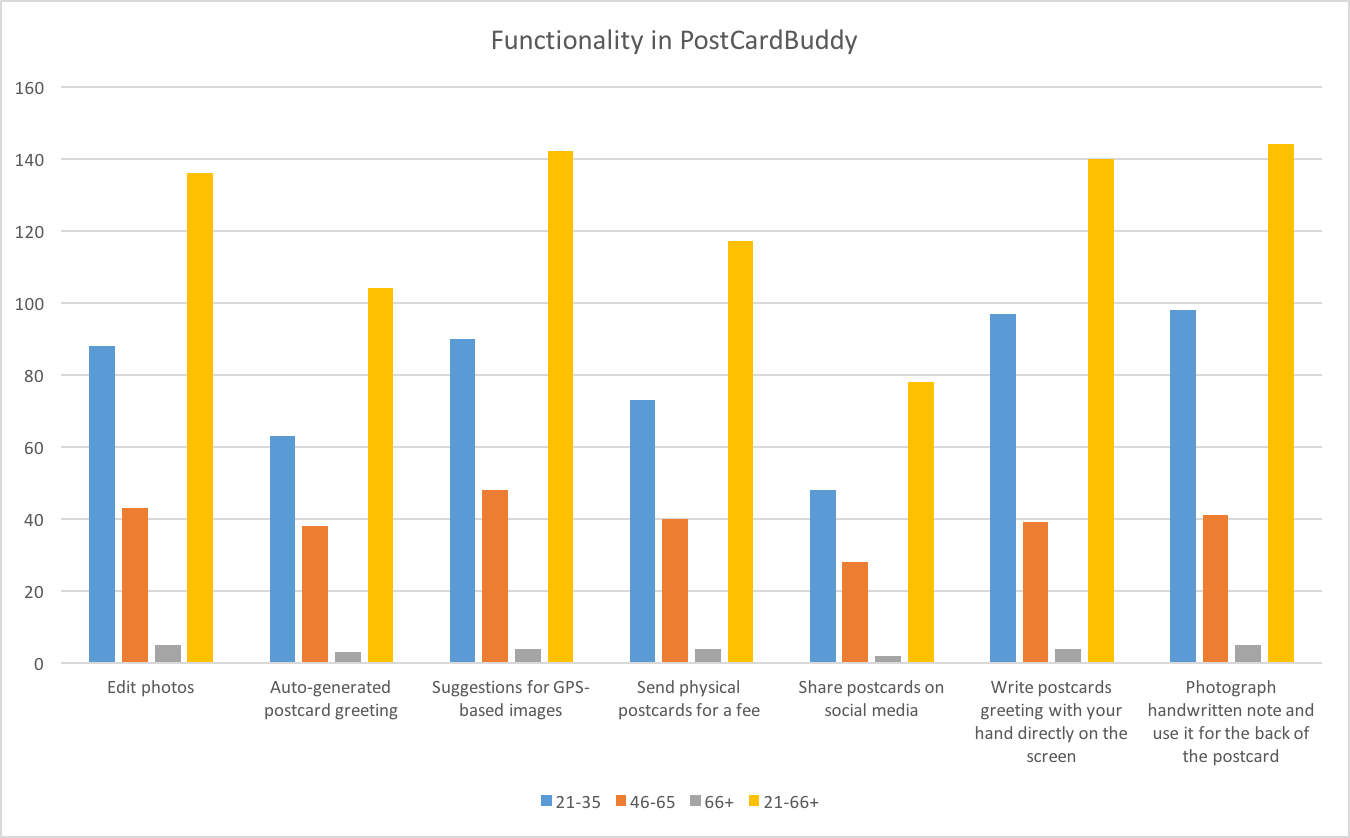
\includegraphics[width=1.0\textwidth]{questionnaire.png}
\caption{Result of the questionnaire on the desired functionality in PostCardBuddy}
\label{fig:questionnaire}
\end{figure}
% Ska vi �ven ha en figur som presenterar hur m�nga 0,1,..5 varje funktion fick???


% 3C) reflect on specification experiences and reason about choices of specification methods in relation to different contexts.
% 5A) combine specification techniques in an explicitly motivated trade off between qualities and costs, where a high degree of specification completeness is achieved for a carefully selected subset of requirements.
\subsection{Specification}
\begin{description}
\item[Context diagram] The first context diagram created is presented in PMv2. The first diagram is very limited and contains too little information to understand the system. The updated diagram is presented in release 1 of the report System Requirements. The biggest problem creating a context diagram is that it should be big enough to present important details, but small enough to be able to get a overview of the system. Therefore it is very important to think through which components it should contain, and which should be left out. This difference is often personal, which we noticed during the creation of release 1, which led to some discussion. The most time of the discussion were spend talking about if the back-end should be presented and how the functionality that is used within the mobile should be presented. 

\item[Data model] The data model is a good tool to easily visualize dependencies of different systems and stakeholders. If done  thoroughly it could be used as a good starting point for developers, and in particular database developers. But the more complicated the data model becomes, the harder it gets for non technical personnel to understand it. And in the same way it loses some of its value for developers if it is not thorough enough. This trade off probably means that this technique should be combined with some other tool, such as a data dictionary, to adequately satisfy technical as well as non-technical personnel. 
\end{description}




% 3H) reflect on validation experiences.
% 5E) utilize links among different types of specifications in validation efforts to find and address potentially harmful inconsistencies.
\subsection{Validation}

% 3J) reflect on prioritization experiences.
\subsection{Prioritization}

%--------------------------------------------------------------------%
%------------ Personal Statements -----------------------------------%
%--------------------------------------------------------------------%
% A personal statement by each team member that briefly explains each individual's contributions to the project results.
\section{Personal Statements}

\begin{thebibliography}{99}
\bibitem{soren} 
	Soren Lauesen,
  	\emph{Software Requirements - Styles and Techniques},
  	Pearson Education Limited, 2002


\end{thebibliography}


\end{document}

